\documentclass{article}
\usepackage{amsmath}
\usepackage{booktabs}
\usepackage{graphicx}

\begin{document}

\section*{Regression Model Analysis}

Using the dataset \texttt{Advertising.csv}, we fit the following regression models with program HW2.py :
\[
\text{(1) } sales = \beta_0 + \beta_1 \cdot radio + \epsilon
\]
\[
\text{(2) } sales = \beta_0 + \beta_1 \cdot newspaper + \epsilon
\]

\subsection*{a. Parameter Estimates}
\[
\hat{sales} = 9.3116 + 0.2025 \cdot radio
\]
\[
\hat{sales} = 12.3514 + 0.0547 \cdot newspaper
\]

\subsection*{b. p-values of $\beta_1$}
\[
p_{\text{radio}} = 4.35 \times 10^{-19}, 
\quad
p_{\text{newspaper}} = 0.00115
\]

\subsection*{c. 95\% Confidence Intervals of $\beta_1$}
\[
\beta_{1,\text{radio}} \in [0.1622, \; 0.2427]
\]
\[
\beta_{1,\text{newspaper}} \in [0.0220, \; 0.0874]
\]

\subsection*{d. Hypothesis Test $H_0: \beta_1 = 0$ ($\alpha{} = 0.05$)}
\begin{itemize}
    \item radio: Since the $p$-value is extremely small, we reject $H_0$. .
    \item newspaper: Since $p = 0.00115 < 0.05$, we reject $H_0$. .
\end{itemize}

\subsection*{Summary Table}

\begin{table}[h!]
\centering
\begin{tabular}{@{}lllll@{}}
\toprule
Model & Regression Equation & $\beta_1$ p-value & 95\% CI of $\beta_1$ & Decision \\ \midrule
sales $\sim$ radio & $9.3116 + 0.2025 \cdot radio$ & $4.35 \times 10^{-19}$ & [0.1622, 0.2427] & Reject $H_0$ \\
sales $\sim$ newspaper & $12.3514 + 0.0547 \cdot newspaper$ & 0.00115 & [0.0220, 0.0874] & Reject $H_0$ \\
\bottomrule
\end{tabular}
\end{table}
\begin{figure}
    \centering
    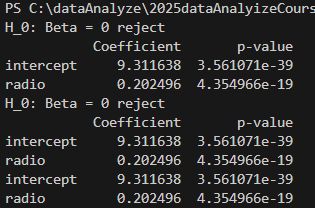
\includegraphics[width=0.5\linewidth]{Homework2_result.png}
    \caption{results on shell}
    \label{fig:placeholder}
\end{figure}
\end{document}
